\documentclass[1p]{elsarticle_modified}
%\bibliographystyle{elsarticle-num}

%\usepackage[colorlinks]{hyperref}
%\usepackage{abbrmath_seonhwa} %\Abb, \Ascr, \Acal ,\Abf, \Afrak
\usepackage{amsfonts}
\usepackage{amssymb}
\usepackage{amsmath}
\usepackage{amsthm}
\usepackage{scalefnt}
\usepackage{amsbsy}
\usepackage{kotex}
\usepackage{caption}
\usepackage{subfig}
\usepackage{color}
\usepackage{graphicx}
\usepackage{xcolor} %% white, black, red, green, blue, cyan, magenta, yellow
\usepackage{float}
\usepackage{setspace}
\usepackage{hyperref}

\usepackage{tikz}
\usetikzlibrary{arrows}

\usepackage{multirow}
\usepackage{array} % fixed length table
\usepackage{hhline}

%%%%%%%%%%%%%%%%%%%%%
\makeatletter
\renewcommand*\env@matrix[1][\arraystretch]{%
	\edef\arraystretch{#1}%
	\hskip -\arraycolsep
	\let\@ifnextchar\new@ifnextchar
	\array{*\c@MaxMatrixCols c}}
\makeatother %https://tex.stackexchange.com/questions/14071/how-can-i-increase-the-line-spacing-in-a-matrix
%%%%%%%%%%%%%%%

\usepackage[normalem]{ulem}

\newcommand{\msout}[1]{\ifmmode\text{\sout{\ensuremath{#1}}}\else\sout{#1}\fi}
%SOURCE: \msout is \stkout macro in https://tex.stackexchange.com/questions/20609/strikeout-in-math-mode

\newcommand{\cancel}[1]{
	\ifmmode
	{\color{red}\msout{#1}}
	\else
	{\color{red}\sout{#1}}
	\fi
}

\newcommand{\add}[1]{
	{\color{blue}\uwave{#1}}
}

\newcommand{\replace}[2]{
	\ifmmode
	{\color{red}\msout{#1}}{\color{blue}\uwave{#2}}
	\else
	{\color{red}\sout{#1}}{\color{blue}\uwave{#2}}
	\fi
}

\newcommand{\Sol}{\mathcal{S}} %segment
\newcommand{\D}{D} %diagram
\newcommand{\A}{\mathcal{A}} %arc


%%%%%%%%%%%%%%%%%%%%%%%%%%%%%5 test

\def\sl{\operatorname{\textup{SL}}(2,\Cbb)}
\def\psl{\operatorname{\textup{PSL}}(2,\Cbb)}
\def\quan{\mkern 1mu \triangleright \mkern 1mu}

\theoremstyle{definition}
\newtheorem{thm}{Theorem}[section]
\newtheorem{prop}[thm]{Proposition}
\newtheorem{lem}[thm]{Lemma}
\newtheorem{ques}[thm]{Question}
\newtheorem{cor}[thm]{Corollary}
\newtheorem{defn}[thm]{Definition}
\newtheorem{exam}[thm]{Example}
\newtheorem{rmk}[thm]{Remark}
\newtheorem{alg}[thm]{Algorithm}

\newcommand{\I}{\sqrt{-1}}
\begin{document}

%\begin{frontmatter}
%
%\title{Boundary parabolic representations of knots up to 8 crossings}
%
%%% Group authors per affiliation:
%\author{Yunhi Cho} 
%\address{Department of Mathematics, University of Seoul, Seoul, Korea}
%\ead{yhcho@uos.ac.kr}
%
%
%\author{Seonhwa Kim} %\fnref{s_kim}}
%\address{Center for Geometry and Physics, Institute for Basic Science, Pohang, 37673, Korea}
%\ead{ryeona17@ibs.re.kr}
%
%\author{Hyuk Kim}
%\address{Department of Mathematical Sciences, Seoul National University, Seoul 08826, Korea}
%\ead{hyukkim@snu.ac.kr}
%
%\author{Seokbeom Yoon}
%\address{Department of Mathematical Sciences, Seoul National University, Seoul, 08826,  Korea}
%\ead{sbyoon15@snu.ac.kr}
%
%\begin{abstract}
%We find all boundary parabolic representation of knots up to 8 crossings.
%
%\end{abstract}
%\begin{keyword}
%    \MSC[2010] 57M25 
%\end{keyword}
%
%\end{frontmatter}

%\linenumbers
%\tableofcontents
%
\newcommand\colored[1]{\textcolor{white}{\rule[-0.35ex]{0.8em}{1.4ex}}\kern-0.8em\color{red} #1}%
%\newcommand\colored[1]{\textcolor{white}{ #1}\kern-2.17ex	\textcolor{white}{ #1}\kern-1.81ex	\textcolor{white}{ #1}\kern-2.15ex\color{red}#1	}

{\Large $\underline{11a_{294}~(K11a_{294})}$}

\setlength{\tabcolsep}{10pt}
\renewcommand{\arraystretch}{1.6}
\vspace{1cm}\begin{tabular}{m{100pt}>{\centering\arraybackslash}m{274pt}}
\multirow{5}{120pt}{
	\centering
	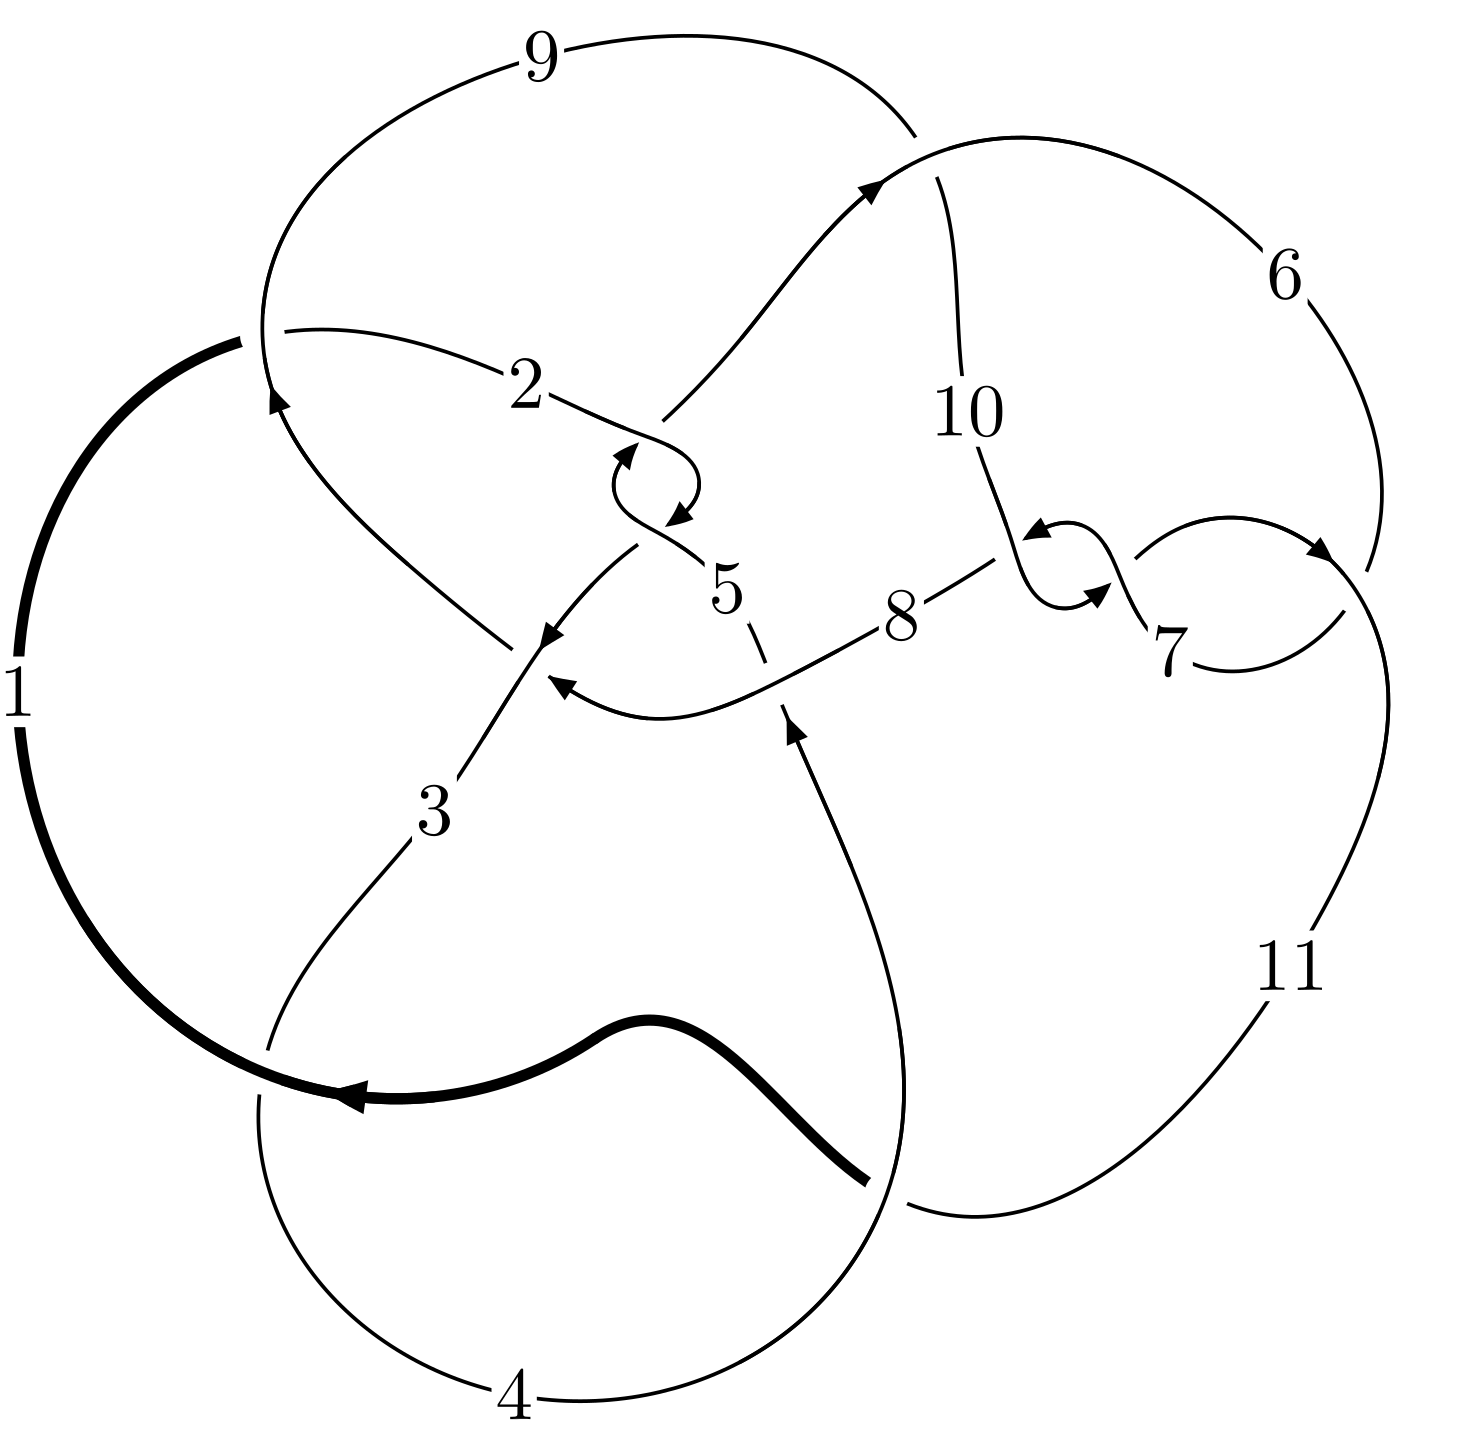
\includegraphics[width=112pt]{../../../GIT/diagram.site/Diagrams/png/543_11a_294.png}\\
\ \ \ A knot diagram\footnotemark}&
\allowdisplaybreaks
\textbf{Linearized knot diagam} \\
\cline{2-2}
 &
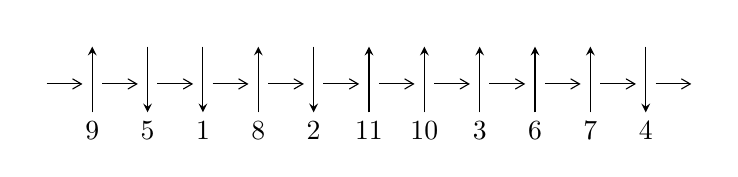
\begin{tikzpicture}[x=20pt, y=17pt]
	% nodes
	\node (C0) at (0, 0) {};
	\node (C1) at (1, 0) {};
	\node (C1U) at (1, +1) {};
	\node (C1D) at (1, -1) {9};

	\node (C2) at (2, 0) {};
	\node (C2U) at (2, +1) {};
	\node (C2D) at (2, -1) {5};

	\node (C3) at (3, 0) {};
	\node (C3U) at (3, +1) {};
	\node (C3D) at (3, -1) {1};

	\node (C4) at (4, 0) {};
	\node (C4U) at (4, +1) {};
	\node (C4D) at (4, -1) {8};

	\node (C5) at (5, 0) {};
	\node (C5U) at (5, +1) {};
	\node (C5D) at (5, -1) {2};

	\node (C6) at (6, 0) {};
	\node (C6U) at (6, +1) {};
	\node (C6D) at (6, -1) {11};

	\node (C7) at (7, 0) {};
	\node (C7U) at (7, +1) {};
	\node (C7D) at (7, -1) {10};

	\node (C8) at (8, 0) {};
	\node (C8U) at (8, +1) {};
	\node (C8D) at (8, -1) {3};

	\node (C9) at (9, 0) {};
	\node (C9U) at (9, +1) {};
	\node (C9D) at (9, -1) {6};

	\node (C10) at (10, 0) {};
	\node (C10U) at (10, +1) {};
	\node (C10D) at (10, -1) {7};

	\node (C11) at (11, 0) {};
	\node (C11U) at (11, +1) {};
	\node (C11D) at (11, -1) {4};
	\node (C12) at (12, 0) {};

	% arrows
	\draw[->,>={angle 60}]
	(C0) edge (C1) (C1) edge (C2) (C2) edge (C3) (C3) edge (C4) (C4) edge (C5) (C5) edge (C6) (C6) edge (C7) (C7) edge (C8) (C8) edge (C9) (C9) edge (C10) (C10) edge (C11) (C11) edge (C12) ;	\draw[->,>=stealth]
	(C1D) edge (C1U) (C2U) edge (C2D) (C3U) edge (C3D) (C4D) edge (C4U) (C5U) edge (C5D) (C6D) edge (C6U) (C7D) edge (C7U) (C8D) edge (C8U) (C9D) edge (C9U) (C10D) edge (C10U) (C11U) edge (C11D) ;
	\end{tikzpicture} \\
\hhline{~~} \\& 
\textbf{Solving Sequence} \\ \cline{2-2} 
 &
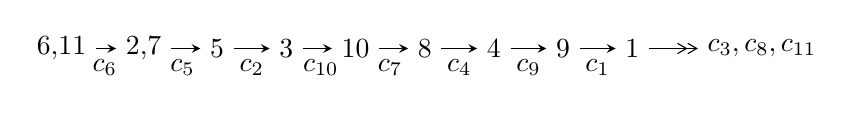
\begin{tikzpicture}[x=25pt, y=7pt]
	% node
	\node (A0) at (-1/8, 0) {6,11};
	\node (A1) at (17/16, 0) {2,7};
	\node (A2) at (17/8, 0) {5};
	\node (A3) at (25/8, 0) {3};
	\node (A4) at (33/8, 0) {10};
	\node (A5) at (41/8, 0) {8};
	\node (A6) at (49/8, 0) {4};
	\node (A7) at (57/8, 0) {9};
	\node (A8) at (65/8, 0) {1};
	\node (C1) at (1/2, -1) {$c_{6}$};
	\node (C2) at (13/8, -1) {$c_{5}$};
	\node (C3) at (21/8, -1) {$c_{2}$};
	\node (C4) at (29/8, -1) {$c_{10}$};
	\node (C5) at (37/8, -1) {$c_{7}$};
	\node (C6) at (45/8, -1) {$c_{4}$};
	\node (C7) at (53/8, -1) {$c_{9}$};
	\node (C8) at (61/8, -1) {$c_{1}$};
	\node (A9) at (10, 0) {$c_{3},c_{8},c_{11}$};

	% edge
	\draw[->,>=stealth]	
	(A0) edge (A1) (A1) edge (A2) (A2) edge (A3) (A3) edge (A4) (A4) edge (A5) (A5) edge (A6) (A6) edge (A7) (A7) edge (A8) ;
	\draw[->>,>={angle 60}]	
	(A8) edge (A9);
\end{tikzpicture} \\ 

\end{tabular} \\

\footnotetext{
The image of knot diagram is generated by the software ``\textbf{Draw programme}" developed by Andrew Bartholomew(\url{http://www.layer8.co.uk/maths/draw/index.htm\#Running-draw}), where we modified some parts for our purpose(\url{https://github.com/CATsTAILs/LinksPainter}).
}\phantom \\ \newline 
\centering \textbf{Ideals for irreducible components\footnotemark of $X_{\text{par}}$} 
 
\begin{align*}
I^u_{1}&=\langle 
-8634895226 u^{23}-5433253456 u^{22}+\cdots+735180934969 b-781237782063,\\
\phantom{I^u_{1}}&\phantom{= \langle  }763967991611 u^{23}+23673073992 u^{22}+\cdots+2940723739876 a+7856566749775,\\
\phantom{I^u_{1}}&\phantom{= \langle  }u^{24}+10 u^{22}+\cdots+15 u-4\rangle \\
I^u_{2}&=\langle 
u^{19} a+2 u^{19}+\cdots-2 a-1,\;-2 u^{19} a-4 u^{19}+\cdots+6 a+15,\;u^{20}- u^{19}+\cdots-2 u-1\rangle \\
I^u_{3}&=\langle 
b+1,\;-2 u^2+2 a-2 u-3,\;u^3+u^2+2 u+1\rangle \\
\\
\end{align*}
\raggedright * 3 irreducible components of $\dim_{\mathbb{C}}=0$, with total 67 representations.\\
\footnotetext{All coefficients of polynomials are rational numbers. But the coefficients are sometimes approximated in decimal forms when there is not enough margin.}
\newpage
\renewcommand{\arraystretch}{1}
\centering \section*{I. $I^u_{1}= \langle -8.63\times10^{9} u^{23}-5.43\times10^{9} u^{22}+\cdots+7.35\times10^{11} b-7.81\times10^{11},\;7.64\times10^{11} u^{23}+2.37\times10^{10} u^{22}+\cdots+2.94\times10^{12} a+7.86\times10^{12},\;u^{24}+10 u^{22}+\cdots+15 u-4 \rangle$}
\flushleft \textbf{(i) Arc colorings}\\
\begin{tabular}{m{7pt} m{180pt} m{7pt} m{180pt} }
\flushright $a_{6}=$&$\begin{pmatrix}1\\0\end{pmatrix}$ \\
\flushright $a_{11}=$&$\begin{pmatrix}0\\u\end{pmatrix}$ \\
\flushright $a_{2}=$&$\begin{pmatrix}-0.259789 u^{23}-0.00805008 u^{22}+\cdots+6.57173 u-2.67164\\0.0117453 u^{23}+0.00739036 u^{22}+\cdots-0.781959 u+1.06265\end{pmatrix}$ \\
\flushright $a_{7}=$&$\begin{pmatrix}1\\- u^2\end{pmatrix}$ \\
\flushright $a_{5}=$&$\begin{pmatrix}0.249773 u^{23}-0.00306836 u^{22}+\cdots-5.95799 u+2.87741\\-0.0126772 u^{23}-0.0249283 u^{22}+\cdots+1.51797 u-1.05571\end{pmatrix}$ \\
\flushright $a_{3}=$&$\begin{pmatrix}-0.517622 u^{23}-0.0138817 u^{22}+\cdots+12.5338 u-5.08757\\0.0138817 u^{23}+0.00372967 u^{22}+\cdots-2.67676 u+2.07049\end{pmatrix}$ \\
\flushright $a_{10}=$&$\begin{pmatrix}- u\\u^3+u\end{pmatrix}$ \\
\flushright $a_{8}=$&$\begin{pmatrix}u^2+1\\- u^4-2 u^2\end{pmatrix}$ \\
\flushright $a_{4}=$&$\begin{pmatrix}0.265662 u^{23}+0.0117453 u^{22}+\cdots-6.46270 u+3.20297\\-0.00805008 u^{23}+0.0403920 u^{22}+\cdots+1.22519 u-1.03916\end{pmatrix}$ \\
\flushright $a_{9}=$&$\begin{pmatrix}- u^3-2 u\\u^3+u\end{pmatrix}$ \\
\flushright $a_{1}=$&$\begin{pmatrix}-0.263929 u^{23}-0.0126772 u^{22}+\cdots+6.43357 u-2.44096\\-0.00306836 u^{23}-0.0138773 u^{22}+\cdots-0.869183 u+0.999092\end{pmatrix}$\\ \flushright $a_{1}=$&$\begin{pmatrix}-0.263929 u^{23}-0.0126772 u^{22}+\cdots+6.43357 u-2.44096\\-0.00306836 u^{23}-0.0138773 u^{22}+\cdots-0.869183 u+0.999092\end{pmatrix}$\\&\end{tabular}
\flushleft \textbf{(ii) Obstruction class $= -1$}\\~\\
\flushleft \textbf{(iii) Cusp Shapes $= \frac{818436095265}{735180934969} u^{23}+\frac{92606395200}{735180934969} u^{22}+\cdots-\frac{104556151676103}{2940723739876} u+\frac{5519991831807}{735180934969}$}\\~\\
\newpage\renewcommand{\arraystretch}{1}
\flushleft \textbf{(iv) u-Polynomials at the component}\newline \\
\begin{tabular}{m{50pt}|m{274pt}}
Crossings & \hspace{64pt}u-Polynomials at each crossing \\
\hline $$\begin{aligned}c_{1},c_{4}\end{aligned}$$&$\begin{aligned}
&8(8 u^{24}-12 u^{23}+\cdots- u+1)
\end{aligned}$\\
\hline $$\begin{aligned}c_{2},c_{3},c_{5}\\c_{11}\end{aligned}$$&$\begin{aligned}
&u^{24}+3 u^{23}+\cdots+6 u-1
\end{aligned}$\\
\hline $$\begin{aligned}c_{6},c_{7},c_{10}\end{aligned}$$&$\begin{aligned}
&u^{24}+10 u^{22}+\cdots-15 u-4
\end{aligned}$\\
\hline $$\begin{aligned}c_{8}\end{aligned}$$&$\begin{aligned}
&u^{24}+3 u^{23}+\cdots+224 u+128
\end{aligned}$\\
\hline $$\begin{aligned}c_{9}\end{aligned}$$&$\begin{aligned}
&u^{24}-6 u^{22}+\cdots-1079 u-676
\end{aligned}$\\
\hline
\end{tabular}\\~\\
\newpage\renewcommand{\arraystretch}{1}
\flushleft \textbf{(v) Riley Polynomials at the component}\newline \\
\begin{tabular}{m{50pt}|m{274pt}}
Crossings & \hspace{64pt}Riley Polynomials at each crossing \\
\hline $$\begin{aligned}c_{1},c_{4}\end{aligned}$$&$\begin{aligned}
&64(64 y^{24}-656 y^{23}+\cdots-7 y+1)
\end{aligned}$\\
\hline $$\begin{aligned}c_{2},c_{3},c_{5}\\c_{11}\end{aligned}$$&$\begin{aligned}
&y^{24}+13 y^{23}+\cdots-38 y+1
\end{aligned}$\\
\hline $$\begin{aligned}c_{6},c_{7},c_{10}\end{aligned}$$&$\begin{aligned}
&y^{24}+20 y^{23}+\cdots-97 y+16
\end{aligned}$\\
\hline $$\begin{aligned}c_{8}\end{aligned}$$&$\begin{aligned}
&y^{24}-7 y^{23}+\cdots-226304 y+16384
\end{aligned}$\\
\hline $$\begin{aligned}c_{9}\end{aligned}$$&$\begin{aligned}
&y^{24}-12 y^{23}+\cdots-1380561 y+456976
\end{aligned}$\\
\hline
\end{tabular}\\~\\
\newpage\flushleft \textbf{(vi) Complex Volumes and Cusp Shapes}
$$\begin{array}{c|c|c}  
\text{Solutions to }I^u_{1}& \I (\text{vol} + \sqrt{-1}CS) & \text{Cusp shape}\\
 \hline 
\begin{aligned}
u &= -1.021460 + 0.275515 I \\
a &= \phantom{-}0.39552 - 1.65501 I \\
b &= \phantom{-}0.047276 + 1.186360 I\end{aligned}
 & \phantom{-}7.49230 - 1.49785 I & \phantom{-}16.5794 + 3.5131 I \\ \hline\begin{aligned}
u &= -1.021460 - 0.275515 I \\
a &= \phantom{-}0.39552 + 1.65501 I \\
b &= \phantom{-}0.047276 - 1.186360 I\end{aligned}
 & \phantom{-}7.49230 + 1.49785 I & \phantom{-}16.5794 - 3.5131 I \\ \hline\begin{aligned}
u &= \phantom{-}0.870278 + 0.206907 I \\
a &= -0.50041 - 2.31304 I \\
b &= -0.49469 + 1.37599 I\end{aligned}
 & \phantom{-}9.3482 + 11.6156 I & \phantom{-}9.04984 - 7.14425 I \\ \hline\begin{aligned}
u &= \phantom{-}0.870278 - 0.206907 I \\
a &= -0.50041 + 2.31304 I \\
b &= -0.49469 - 1.37599 I\end{aligned}
 & \phantom{-}9.3482 - 11.6156 I & \phantom{-}9.04984 + 7.14425 I \\ \hline\begin{aligned}
u &= -0.711520 + 0.880248 I \\
a &= -0.496210 + 1.180490 I \\
b &= -0.138302 - 1.193200 I\end{aligned}
 & \phantom{-}5.61526 - 4.36903 I & \phantom{-}11.9512 + 7.5869 I \\ \hline\begin{aligned}
u &= -0.711520 - 0.880248 I \\
a &= -0.496210 - 1.180490 I \\
b &= -0.138302 + 1.193200 I\end{aligned}
 & \phantom{-}5.61526 + 4.36903 I & \phantom{-}11.9512 - 7.5869 I \\ \hline\begin{aligned}
u &= \phantom{-}0.507475 + 1.020800 I \\
a &= \phantom{-}0.471884 + 1.006850 I \\
b &= -0.411983 - 1.346680 I\end{aligned}
 & \phantom{-}6.85359 - 6.74871 I & \phantom{-}7.12828 + 3.44529 I \\ \hline\begin{aligned}
u &= \phantom{-}0.507475 - 1.020800 I \\
a &= \phantom{-}0.471884 - 1.006850 I \\
b &= -0.411983 + 1.346680 I\end{aligned}
 & \phantom{-}6.85359 + 6.74871 I & \phantom{-}7.12828 - 3.44529 I \\ \hline\begin{aligned}
u &= \phantom{-}0.263649 + 1.293920 I \\
a &= \phantom{-}0.137301 + 0.951214 I \\
b &= \phantom{-}1.347430 + 0.188650 I\end{aligned}
 & -4.17750 + 3.32302 I & \phantom{-}7.49326 - 7.01534 I \\ \hline\begin{aligned}
u &= \phantom{-}0.263649 - 1.293920 I \\
a &= \phantom{-}0.137301 - 0.951214 I \\
b &= \phantom{-}1.347430 - 0.188650 I\end{aligned}
 & -4.17750 - 3.32302 I & \phantom{-}7.49326 + 7.01534 I\\
 \hline 
 \end{array}$$\newpage$$\begin{array}{c|c|c}  
\text{Solutions to }I^u_{1}& \I (\text{vol} + \sqrt{-1}CS) & \text{Cusp shape}\\
 \hline 
\begin{aligned}
u &= \phantom{-}0.102906 + 1.325920 I \\
a &= \phantom{-}0.978679 + 0.749632 I \\
b &= \phantom{-}0.912691 - 0.587846 I\end{aligned}
 & -5.99931 + 2.29383 I & -3.48033 - 0.30083 I \\ \hline\begin{aligned}
u &= \phantom{-}0.102906 - 1.325920 I \\
a &= \phantom{-}0.978679 - 0.749632 I \\
b &= \phantom{-}0.912691 + 0.587846 I\end{aligned}
 & -5.99931 - 2.29383 I & -3.48033 + 0.30083 I \\ \hline\begin{aligned}
u &= \phantom{-}0.656566\phantom{ +0.000000I} \\
a &= -1.48947\phantom{ +0.000000I} \\
b &= \phantom{-}1.29551\phantom{ +0.000000I}\end{aligned}
 & -0.112715\phantom{ +0.000000I} & \phantom{-}17.2960\phantom{ +0.000000I} \\ \hline\begin{aligned}
u &= -0.181673 + 1.332990 I \\
a &= -0.477910 + 0.021115 I \\
b &= -0.263704 + 0.229700 I\end{aligned}
 & -3.41691 - 2.41506 I & \phantom{-}4.35202 + 1.54076 I \\ \hline\begin{aligned}
u &= -0.181673 - 1.332990 I \\
a &= -0.477910 - 0.021115 I \\
b &= -0.263704 - 0.229700 I\end{aligned}
 & -3.41691 + 2.41506 I & \phantom{-}4.35202 - 1.54076 I \\ \hline\begin{aligned}
u &= \phantom{-}0.36901 + 1.39774 I \\
a &= -1.48756 - 1.23046 I \\
b &= -0.55509 + 1.37302 I\end{aligned}
 & \phantom{-}4.2704 + 16.0735 I & \phantom{-}4.86533 - 8.67439 I \\ \hline\begin{aligned}
u &= \phantom{-}0.36901 - 1.39774 I \\
a &= -1.48756 + 1.23046 I \\
b &= -0.55509 - 1.37302 I\end{aligned}
 & \phantom{-}4.2704 - 16.0735 I & \phantom{-}4.86533 + 8.67439 I \\ \hline\begin{aligned}
u &= -0.45316 + 1.40935 I \\
a &= \phantom{-}0.831561 - 1.018120 I \\
b &= \phantom{-}0.207861 + 1.159740 I\end{aligned}
 & \phantom{-}2.26090 - 6.77325 I & \phantom{-}8.15326 + 8.68487 I \\ \hline\begin{aligned}
u &= -0.45316 - 1.40935 I \\
a &= \phantom{-}0.831561 + 1.018120 I \\
b &= \phantom{-}0.207861 - 1.159740 I\end{aligned}
 & \phantom{-}2.26090 + 6.77325 I & \phantom{-}8.15326 - 8.68487 I \\ \hline\begin{aligned}
u &= -0.496850\phantom{ +0.000000I} \\
a &= -0.482259\phantom{ +0.000000I} \\
b &= -0.161437\phantom{ +0.000000I}\end{aligned}
 & \phantom{-}0.853473\phantom{ +0.000000I} & \phantom{-}12.2560\phantom{ +0.000000I}\\
 \hline 
 \end{array}$$\newpage$$\begin{array}{c|c|c}  
\text{Solutions to }I^u_{1}& \I (\text{vol} + \sqrt{-1}CS) & \text{Cusp shape}\\
 \hline 
\begin{aligned}
u &= -0.11292 + 1.52095 I \\
a &= -0.621242 + 0.178604 I \\
b &= -0.381421 - 1.074640 I\end{aligned}
 & -2.48001 - 6.89114 I & \phantom{-}2.89593 + 8.03535 I \\ \hline\begin{aligned}
u &= -0.11292 - 1.52095 I \\
a &= -0.621242 - 0.178604 I \\
b &= -0.381421 + 1.074640 I\end{aligned}
 & -2.48001 + 6.89114 I & \phantom{-}2.89593 - 8.03535 I \\ \hline\begin{aligned}
u &= \phantom{-}0.287554 + 0.235788 I \\
a &= -0.37075 + 1.66780 I \\
b &= \phantom{-}0.662890 - 0.292141 I\end{aligned}
 & -1.22051 + 0.86188 I & -4.63925 - 4.32694 I \\ \hline\begin{aligned}
u &= \phantom{-}0.287554 - 0.235788 I \\
a &= -0.37075 - 1.66780 I \\
b &= \phantom{-}0.662890 + 0.292141 I\end{aligned}
 & -1.22051 - 0.86188 I & -4.63925 + 4.32694 I\\
 \hline 
 \end{array}$$\newpage\newpage\renewcommand{\arraystretch}{1}
\centering \section*{II. $I^u_{2}= \langle u^{19} a+2 u^{19}+\cdots-2 a-1,\;-2 u^{19} a-4 u^{19}+\cdots+6 a+15,\;u^{20}- u^{19}+\cdots-2 u-1 \rangle$}
\flushleft \textbf{(i) Arc colorings}\\
\begin{tabular}{m{7pt} m{180pt} m{7pt} m{180pt} }
\flushright $a_{6}=$&$\begin{pmatrix}1\\0\end{pmatrix}$ \\
\flushright $a_{11}=$&$\begin{pmatrix}0\\u\end{pmatrix}$ \\
\flushright $a_{2}=$&$\begin{pmatrix}a\\- u^{19} a-2 u^{19}+\cdots+2 a+1\end{pmatrix}$ \\
\flushright $a_{7}=$&$\begin{pmatrix}1\\- u^2\end{pmatrix}$ \\
\flushright $a_{5}=$&$\begin{pmatrix}-2 u^{19} a-4 u^{19}+\cdots+a+7\\u^{19} a- u^{19}+\cdots+2 a+3\end{pmatrix}$ \\
\flushright $a_{3}=$&$\begin{pmatrix}- u^{19}-8 u^{17}-26 u^{15}-42 u^{13}-31 u^{11}-2 u^9+10 u^7+4 u^5- u^3-2 u\\u^{19}- u^{18}+\cdots+2 u+1\end{pmatrix}$ \\
\flushright $a_{10}=$&$\begin{pmatrix}- u\\u^3+u\end{pmatrix}$ \\
\flushright $a_{8}=$&$\begin{pmatrix}u^2+1\\- u^4-2 u^2\end{pmatrix}$ \\
\flushright $a_{4}=$&$\begin{pmatrix}-2 u^{19} a- u^{19}+\cdots-7 u+3\\-2 u^{19}+2 u^{18}+\cdots-2 u+2\end{pmatrix}$ \\
\flushright $a_{9}=$&$\begin{pmatrix}- u^3-2 u\\u^3+u\end{pmatrix}$ \\
\flushright $a_{1}=$&$\begin{pmatrix}-2 u^{19} a- u^{19}+\cdots+2 a-2\\- u^{18} a-2 u^{19}+\cdots+2 a+2\end{pmatrix}$\\ \flushright $a_{1}=$&$\begin{pmatrix}-2 u^{19} a- u^{19}+\cdots+2 a-2\\- u^{18} a-2 u^{19}+\cdots+2 a+2\end{pmatrix}$\\&\end{tabular}
\flushleft \textbf{(ii) Obstruction class $= -1$}\\~\\
\flushleft \textbf{(iii) Cusp Shapes $= 4 u^{18}-4 u^{17}+32 u^{16}-28 u^{15}+104 u^{14}-76 u^{13}+164 u^{12}-92 u^{11}+104 u^{10}-32 u^9-28 u^8+20 u^7-60 u^6+4 u^5-4 u^4-8 u^3+16 u^2+4 u+10$}\\~\\
\newpage\renewcommand{\arraystretch}{1}
\flushleft \textbf{(iv) u-Polynomials at the component}\newline \\
\begin{tabular}{m{50pt}|m{274pt}}
Crossings & \hspace{64pt}u-Polynomials at each crossing \\
\hline $$\begin{aligned}c_{1},c_{4}\end{aligned}$$&$\begin{aligned}
&u^{40}-3 u^{39}+\cdots-60100 u+13049
\end{aligned}$\\
\hline $$\begin{aligned}c_{2},c_{3},c_{5}\\c_{11}\end{aligned}$$&$\begin{aligned}
&u^{40}-7 u^{39}+\cdots-2 u+1
\end{aligned}$\\
\hline $$\begin{aligned}c_{6},c_{7},c_{10}\end{aligned}$$&$\begin{aligned}
&(u^{20}+u^{19}+\cdots+2 u-1)^{2}
\end{aligned}$\\
\hline $$\begin{aligned}c_{8}\end{aligned}$$&$\begin{aligned}
&(u^{20}- u^{19}+\cdots+3 u^2-1)^{2}
\end{aligned}$\\
\hline $$\begin{aligned}c_{9}\end{aligned}$$&$\begin{aligned}
&(u^{20}- u^{19}+\cdots+4 u-1)^{2}
\end{aligned}$\\
\hline
\end{tabular}\\~\\
\newpage\renewcommand{\arraystretch}{1}
\flushleft \textbf{(v) Riley Polynomials at the component}\newline \\
\begin{tabular}{m{50pt}|m{274pt}}
Crossings & \hspace{64pt}Riley Polynomials at each crossing \\
\hline $$\begin{aligned}c_{1},c_{4}\end{aligned}$$&$\begin{aligned}
&y^{40}-21 y^{39}+\cdots-1779930400 y+170276401
\end{aligned}$\\
\hline $$\begin{aligned}c_{2},c_{3},c_{5}\\c_{11}\end{aligned}$$&$\begin{aligned}
&y^{40}+27 y^{39}+\cdots+40 y^2+1
\end{aligned}$\\
\hline $$\begin{aligned}c_{6},c_{7},c_{10}\end{aligned}$$&$\begin{aligned}
&(y^{20}+17 y^{19}+\cdots-6 y+1)^{2}
\end{aligned}$\\
\hline $$\begin{aligned}c_{8}\end{aligned}$$&$\begin{aligned}
&(y^{20}-7 y^{19}+\cdots-6 y+1)^{2}
\end{aligned}$\\
\hline $$\begin{aligned}c_{9}\end{aligned}$$&$\begin{aligned}
&(y^{20}-11 y^{19}+\cdots-6 y+1)^{2}
\end{aligned}$\\
\hline
\end{tabular}\\~\\
\newpage\flushleft \textbf{(vi) Complex Volumes and Cusp Shapes}
$$\begin{array}{c|c|c}  
\text{Solutions to }I^u_{2}& \I (\text{vol} + \sqrt{-1}CS) & \text{Cusp shape}\\
 \hline 
\begin{aligned}
u &= \phantom{-}0.274747 + 1.069600 I \\
a &= -0.650977 - 1.009380 I \\
b &= \phantom{-}0.31766 + 1.39547 I\end{aligned}
 & \phantom{-}2.02098 - 2.13456 I & \phantom{-}4.50898 + 2.16962 I \\ \hline\begin{aligned}
u &= \phantom{-}0.274747 + 1.069600 I \\
a &= -0.084213 - 0.753588 I \\
b &= -0.918130 - 0.259874 I\end{aligned}
 & \phantom{-}2.02098 - 2.13456 I & \phantom{-}4.50898 + 2.16962 I \\ \hline\begin{aligned}
u &= \phantom{-}0.274747 - 1.069600 I \\
a &= -0.650977 + 1.009380 I \\
b &= \phantom{-}0.31766 - 1.39547 I\end{aligned}
 & \phantom{-}2.02098 + 2.13456 I & \phantom{-}4.50898 - 2.16962 I \\ \hline\begin{aligned}
u &= \phantom{-}0.274747 - 1.069600 I \\
a &= -0.084213 + 0.753588 I \\
b &= -0.918130 + 0.259874 I\end{aligned}
 & \phantom{-}2.02098 + 2.13456 I & \phantom{-}4.50898 - 2.16962 I \\ \hline\begin{aligned}
u &= \phantom{-}0.773104 + 0.153161 I \\
a &= \phantom{-}0.829907 - 0.370587 I \\
b &= -1.084140 + 0.080482 I\end{aligned}
 & \phantom{-}4.77271 + 6.07240 I & \phantom{-}7.45285 - 5.87540 I \\ \hline\begin{aligned}
u &= \phantom{-}0.773104 + 0.153161 I \\
a &= \phantom{-}0.37153 + 2.57431 I \\
b &= \phantom{-}0.49433 - 1.41099 I\end{aligned}
 & \phantom{-}4.77271 + 6.07240 I & \phantom{-}7.45285 - 5.87540 I \\ \hline\begin{aligned}
u &= \phantom{-}0.773104 - 0.153161 I \\
a &= \phantom{-}0.829907 + 0.370587 I \\
b &= -1.084140 - 0.080482 I\end{aligned}
 & \phantom{-}4.77271 - 6.07240 I & \phantom{-}7.45285 + 5.87540 I \\ \hline\begin{aligned}
u &= \phantom{-}0.773104 - 0.153161 I \\
a &= \phantom{-}0.37153 - 2.57431 I \\
b &= \phantom{-}0.49433 + 1.41099 I\end{aligned}
 & \phantom{-}4.77271 - 6.07240 I & \phantom{-}7.45285 + 5.87540 I \\ \hline\begin{aligned}
u &= \phantom{-}0.772326\phantom{ +0.000000I} \\
a &= \phantom{-}0.10498 + 2.42938 I \\
b &= -0.56866 - 1.40361 I\end{aligned}
 & \phantom{-}8.84775\phantom{ +0.000000I} & \phantom{-}12.4400\phantom{ +0.000000I} \\ \hline\begin{aligned}
u &= \phantom{-}0.772326\phantom{ +0.000000I} \\
a &= \phantom{-}0.10498 - 2.42938 I \\
b &= -0.56866 + 1.40361 I\end{aligned}
 & \phantom{-}8.84775\phantom{ +0.000000I} & \phantom{-}12.4400\phantom{ +0.000000I}\\
 \hline 
 \end{array}$$\newpage$$\begin{array}{c|c|c}  
\text{Solutions to }I^u_{2}& \I (\text{vol} + \sqrt{-1}CS) & \text{Cusp shape}\\
 \hline 
\begin{aligned}
u &= -0.198534 + 1.239650 I \\
a &= \phantom{-}1.83297 - 0.91329 I \\
b &= \phantom{-}0.199750 - 0.784968 I\end{aligned}
 & \phantom{-}0.52569 - 2.16136 I & \phantom{-}0.73748 + 3.31855 I \\ \hline\begin{aligned}
u &= -0.198534 + 1.239650 I \\
a &= \phantom{-}0.01849 - 2.83921 I \\
b &= \phantom{-}0.053071 + 1.161370 I\end{aligned}
 & \phantom{-}0.52569 - 2.16136 I & \phantom{-}0.73748 + 3.31855 I \\ \hline\begin{aligned}
u &= -0.198534 - 1.239650 I \\
a &= \phantom{-}1.83297 + 0.91329 I \\
b &= \phantom{-}0.199750 + 0.784968 I\end{aligned}
 & \phantom{-}0.52569 + 2.16136 I & \phantom{-}0.73748 - 3.31855 I \\ \hline\begin{aligned}
u &= -0.198534 - 1.239650 I \\
a &= \phantom{-}0.01849 + 2.83921 I \\
b &= \phantom{-}0.053071 - 1.161370 I\end{aligned}
 & \phantom{-}0.52569 + 2.16136 I & \phantom{-}0.73748 - 3.31855 I \\ \hline\begin{aligned}
u &= -0.692333 + 0.156175 I \\
a &= \phantom{-}0.333781 + 0.644615 I \\
b &= \phantom{-}0.162072 + 0.252940 I\end{aligned}
 & \phantom{-}3.61438 - 0.81573 I & \phantom{-}5.67172 + 1.07888 I \\ \hline\begin{aligned}
u &= -0.692333 + 0.156175 I \\
a &= -1.37017 + 2.40156 I \\
b &= -0.049861 - 1.112720 I\end{aligned}
 & \phantom{-}3.61438 - 0.81573 I & \phantom{-}5.67172 + 1.07888 I \\ \hline\begin{aligned}
u &= -0.692333 - 0.156175 I \\
a &= \phantom{-}0.333781 - 0.644615 I \\
b &= \phantom{-}0.162072 - 0.252940 I\end{aligned}
 & \phantom{-}3.61438 + 0.81573 I & \phantom{-}5.67172 - 1.07888 I \\ \hline\begin{aligned}
u &= -0.692333 - 0.156175 I \\
a &= -1.37017 - 2.40156 I \\
b &= -0.049861 + 1.112720 I\end{aligned}
 & \phantom{-}3.61438 + 0.81573 I & \phantom{-}5.67172 - 1.07888 I \\ \hline\begin{aligned}
u &= \phantom{-}0.327541 + 1.260030 I \\
a &= \phantom{-}0.653810 + 0.673934 I \\
b &= -0.46464 - 1.49110 I\end{aligned}
 & \phantom{-}4.94645 + 3.96853 I & \phantom{-}7.89349 - 3.79787 I \\ \hline\begin{aligned}
u &= \phantom{-}0.327541 + 1.260030 I \\
a &= -1.51060 - 1.23935 I \\
b &= -0.67909 + 1.31567 I\end{aligned}
 & \phantom{-}4.94645 + 3.96853 I & \phantom{-}7.89349 - 3.79787 I\\
 \hline 
 \end{array}$$\newpage$$\begin{array}{c|c|c}  
\text{Solutions to }I^u_{2}& \I (\text{vol} + \sqrt{-1}CS) & \text{Cusp shape}\\
 \hline 
\begin{aligned}
u &= \phantom{-}0.327541 - 1.260030 I \\
a &= \phantom{-}0.653810 - 0.673934 I \\
b &= -0.46464 + 1.49110 I\end{aligned}
 & \phantom{-}4.94645 - 3.96853 I & \phantom{-}7.89349 + 3.79787 I \\ \hline\begin{aligned}
u &= \phantom{-}0.327541 - 1.260030 I \\
a &= -1.51060 + 1.23935 I \\
b &= -0.67909 - 1.31567 I\end{aligned}
 & \phantom{-}4.94645 - 3.96853 I & \phantom{-}7.89349 + 3.79787 I \\ \hline\begin{aligned}
u &= -0.201509 + 0.663357 I \\
a &= -0.408683 - 0.835639 I \\
b &= -0.502025 - 0.160176 I\end{aligned}
 & \phantom{-}1.62333 - 2.35832 I & \phantom{-}2.35225 + 4.49783 I \\ \hline\begin{aligned}
u &= -0.201509 + 0.663357 I \\
a &= \phantom{-}0.005727 - 0.731461 I \\
b &= \phantom{-}0.195325 + 1.163080 I\end{aligned}
 & \phantom{-}1.62333 - 2.35832 I & \phantom{-}2.35225 + 4.49783 I \\ \hline\begin{aligned}
u &= -0.201509 - 0.663357 I \\
a &= -0.408683 + 0.835639 I \\
b &= -0.502025 + 0.160176 I\end{aligned}
 & \phantom{-}1.62333 + 2.35832 I & \phantom{-}2.35225 - 4.49783 I \\ \hline\begin{aligned}
u &= -0.201509 - 0.663357 I \\
a &= \phantom{-}0.005727 + 0.731461 I \\
b &= \phantom{-}0.195325 - 1.163080 I\end{aligned}
 & \phantom{-}1.62333 + 2.35832 I & \phantom{-}2.35225 - 4.49783 I \\ \hline\begin{aligned}
u &= -0.295567 + 1.352050 I \\
a &= \phantom{-}0.356054 + 0.330760 I \\
b &= \phantom{-}0.392505 + 0.067994 I\end{aligned}
 & -1.14075 - 4.43308 I & \phantom{-}0.68370 + 2.52728 I \\ \hline\begin{aligned}
u &= -0.295567 + 1.352050 I \\
a &= -1.53457 + 1.07334 I \\
b &= -0.177275 - 1.088720 I\end{aligned}
 & -1.14075 - 4.43308 I & \phantom{-}0.68370 + 2.52728 I \\ \hline\begin{aligned}
u &= -0.295567 - 1.352050 I \\
a &= \phantom{-}0.356054 - 0.330760 I \\
b &= \phantom{-}0.392505 - 0.067994 I\end{aligned}
 & -1.14075 + 4.43308 I & \phantom{-}0.68370 - 2.52728 I \\ \hline\begin{aligned}
u &= -0.295567 - 1.352050 I \\
a &= -1.53457 - 1.07334 I \\
b &= -0.177275 + 1.088720 I\end{aligned}
 & -1.14075 + 4.43308 I & \phantom{-}0.68370 - 2.52728 I\\
 \hline 
 \end{array}$$\newpage$$\begin{array}{c|c|c}  
\text{Solutions to }I^u_{2}& \I (\text{vol} + \sqrt{-1}CS) & \text{Cusp shape}\\
 \hline 
\begin{aligned}
u &= \phantom{-}0.328206 + 1.357610 I \\
a &= -0.283063 - 0.801762 I \\
b &= -1.159930 - 0.023595 I\end{aligned}
 & \phantom{-}0.00745 + 10.05770 I & \phantom{-}2.70834 - 7.26612 I \\ \hline\begin{aligned}
u &= \phantom{-}0.328206 + 1.357610 I \\
a &= \phantom{-}1.50051 + 1.23763 I \\
b &= \phantom{-}0.59445 - 1.40555 I\end{aligned}
 & \phantom{-}0.00745 + 10.05770 I & \phantom{-}2.70834 - 7.26612 I \\ \hline\begin{aligned}
u &= \phantom{-}0.328206 - 1.357610 I \\
a &= -0.283063 + 0.801762 I \\
b &= -1.159930 + 0.023595 I\end{aligned}
 & \phantom{-}0.00745 - 10.05770 I & \phantom{-}2.70834 + 7.26612 I \\ \hline\begin{aligned}
u &= \phantom{-}0.328206 - 1.357610 I \\
a &= \phantom{-}1.50051 - 1.23763 I \\
b &= \phantom{-}0.59445 + 1.40555 I\end{aligned}
 & \phantom{-}0.00745 - 10.05770 I & \phantom{-}2.70834 + 7.26612 I \\ \hline\begin{aligned}
u &= -0.022410 + 1.403750 I \\
a &= -0.788895 - 0.405125 I \\
b &= -0.676901 + 0.349305 I\end{aligned}
 & -4.68486 - 2.84648 I & -1.60998 + 2.97861 I \\ \hline\begin{aligned}
u &= -0.022410 + 1.403750 I \\
a &= \phantom{-}0.387309 + 0.213744 I \\
b &= \phantom{-}0.495392 + 0.955288 I\end{aligned}
 & -4.68486 - 2.84648 I & -1.60998 + 2.97861 I \\ \hline\begin{aligned}
u &= -0.022410 - 1.403750 I \\
a &= -0.788895 + 0.405125 I \\
b &= -0.676901 - 0.349305 I\end{aligned}
 & -4.68486 + 2.84648 I & -1.60998 - 2.97861 I \\ \hline\begin{aligned}
u &= -0.022410 - 1.403750 I \\
a &= \phantom{-}0.387309 - 0.213744 I \\
b &= \phantom{-}0.495392 - 0.955288 I\end{aligned}
 & -4.68486 + 2.84648 I & -1.60998 - 2.97861 I \\ \hline\begin{aligned}
u &= -0.358818\phantom{ +0.000000I} \\
a &= -4.26389 + 1.88679 I \\
b &= -0.123906 + 1.022770 I\end{aligned}
 & \phantom{-}3.97005\phantom{ +0.000000I} & \phantom{-}10.7620\phantom{ +0.000000I} \\ \hline\begin{aligned}
u &= -0.358818\phantom{ +0.000000I} \\
a &= -4.26389 - 1.88679 I \\
b &= -0.123906 - 1.022770 I\end{aligned}
 & \phantom{-}3.97005\phantom{ +0.000000I} & \phantom{-}10.7620\phantom{ +0.000000I}\\
 \hline 
 \end{array}$$\newpage\newpage\renewcommand{\arraystretch}{1}
\centering \section*{III. $I^u_{3}= \langle b+1,\;-2 u^2+2 a-2 u-3,\;u^3+u^2+2 u+1 \rangle$}
\flushleft \textbf{(i) Arc colorings}\\
\begin{tabular}{m{7pt} m{180pt} m{7pt} m{180pt} }
\flushright $a_{6}=$&$\begin{pmatrix}1\\0\end{pmatrix}$ \\
\flushright $a_{11}=$&$\begin{pmatrix}0\\u\end{pmatrix}$ \\
\flushright $a_{2}=$&$\begin{pmatrix}u^2+u+\frac{3}{2}\\-1\end{pmatrix}$ \\
\flushright $a_{7}=$&$\begin{pmatrix}1\\- u^2\end{pmatrix}$ \\
\flushright $a_{5}=$&$\begin{pmatrix}u^2+u+\frac{5}{2}\\-1\end{pmatrix}$ \\
\flushright $a_{3}=$&$\begin{pmatrix}2 u^2+2 u+4\\-2\end{pmatrix}$ \\
\flushright $a_{10}=$&$\begin{pmatrix}- u\\- u^2- u-1\end{pmatrix}$ \\
\flushright $a_{8}=$&$\begin{pmatrix}u^2+1\\- u^2- u-1\end{pmatrix}$ \\
\flushright $a_{4}=$&$\begin{pmatrix}u^2+u+2\\-\frac{1}{2} u-1\end{pmatrix}$ \\
\flushright $a_{9}=$&$\begin{pmatrix}u^2+1\\- u^2- u-1\end{pmatrix}$ \\
\flushright $a_{1}=$&$\begin{pmatrix}u^2+u+2\\\frac{1}{2} u-1\end{pmatrix}$\\ \flushright $a_{1}=$&$\begin{pmatrix}u^2+u+2\\\frac{1}{2} u-1\end{pmatrix}$\\&\end{tabular}
\flushleft \textbf{(ii) Obstruction class $= 1$}\\~\\
\flushleft \textbf{(iii) Cusp Shapes $= \frac{1}{4} u-2$}\\~\\
\newpage\renewcommand{\arraystretch}{1}
\flushleft \textbf{(iv) u-Polynomials at the component}\newline \\
\begin{tabular}{m{50pt}|m{274pt}}
Crossings & \hspace{64pt}u-Polynomials at each crossing \\
\hline $$\begin{aligned}c_{1}\end{aligned}$$&$\begin{aligned}
&8(8 u^3+4 u^2-1)
\end{aligned}$\\
\hline $$\begin{aligned}c_{2},c_{11}\end{aligned}$$&$\begin{aligned}
&(u-1)^3
\end{aligned}$\\
\hline $$\begin{aligned}c_{3},c_{5}\end{aligned}$$&$\begin{aligned}
&(u+1)^3
\end{aligned}$\\
\hline $$\begin{aligned}c_{4}\end{aligned}$$&$\begin{aligned}
&8(8 u^3-4 u^2+1)
\end{aligned}$\\
\hline $$\begin{aligned}c_{6},c_{7}\end{aligned}$$&$\begin{aligned}
&u^3+u^2+2 u+1
\end{aligned}$\\
\hline $$\begin{aligned}c_{8}\end{aligned}$$&$\begin{aligned}
&u^3
\end{aligned}$\\
\hline $$\begin{aligned}c_{9}\end{aligned}$$&$\begin{aligned}
&u^3+u^2-1
\end{aligned}$\\
\hline $$\begin{aligned}c_{10}\end{aligned}$$&$\begin{aligned}
&u^3- u^2+2 u-1
\end{aligned}$\\
\hline
\end{tabular}\\~\\
\newpage\renewcommand{\arraystretch}{1}
\flushleft \textbf{(v) Riley Polynomials at the component}\newline \\
\begin{tabular}{m{50pt}|m{274pt}}
Crossings & \hspace{64pt}Riley Polynomials at each crossing \\
\hline $$\begin{aligned}c_{1},c_{4}\end{aligned}$$&$\begin{aligned}
&64(64 y^3-16 y^2+8 y-1)
\end{aligned}$\\
\hline $$\begin{aligned}c_{2},c_{3},c_{5}\\c_{11}\end{aligned}$$&$\begin{aligned}
&(y-1)^3
\end{aligned}$\\
\hline $$\begin{aligned}c_{6},c_{7},c_{10}\end{aligned}$$&$\begin{aligned}
&y^3+3 y^2+2 y-1
\end{aligned}$\\
\hline $$\begin{aligned}c_{8}\end{aligned}$$&$\begin{aligned}
&y^3
\end{aligned}$\\
\hline $$\begin{aligned}c_{9}\end{aligned}$$&$\begin{aligned}
&y^3- y^2+2 y-1
\end{aligned}$\\
\hline
\end{tabular}\\~\\
\newpage\flushleft \textbf{(vi) Complex Volumes and Cusp Shapes}
$$\begin{array}{c|c|c}  
\text{Solutions to }I^u_{3}& \I (\text{vol} + \sqrt{-1}CS) & \text{Cusp shape}\\
 \hline 
\begin{aligned}
u &= -0.215080 + 1.307140 I \\
a &= -0.377439 + 0.744862 I \\
b &= -1.00000\phantom{ +0.000000I}\end{aligned}
 & -4.66906 - 2.82812 I & -2.05377 + 0.32679 I \\ \hline\begin{aligned}
u &= -0.215080 - 1.307140 I \\
a &= -0.377439 - 0.744862 I \\
b &= -1.00000\phantom{ +0.000000I}\end{aligned}
 & -4.66906 + 2.82812 I & -2.05377 - 0.32679 I \\ \hline\begin{aligned}
u &= -0.569840\phantom{ +0.000000I} \\
a &= \phantom{-}1.25488\phantom{ +0.000000I} \\
b &= -1.00000\phantom{ +0.000000I}\end{aligned}
 & -0.531480\phantom{ +0.000000I} & -2.14250\phantom{ +0.000000I}\\
 \hline 
 \end{array}$$\newpage
\newpage\renewcommand{\arraystretch}{1}
\centering \section*{ IV. u-Polynomials}
\begin{tabular}{m{50pt}|m{274pt}}
Crossings & \hspace{64pt}u-Polynomials at each crossing \\
\hline $$\begin{aligned}c_{1}\end{aligned}$$&$\begin{aligned}
&64(8 u^3+4 u^2-1)(8 u^{24}-12 u^{23}+\cdots- u+1)\\
&\cdot(u^{40}-3 u^{39}+\cdots-60100 u+13049)
\end{aligned}$\\
\hline $$\begin{aligned}c_{2},c_{11}\end{aligned}$$&$\begin{aligned}
&((u-1)^3)(u^{24}+3 u^{23}+\cdots+6 u-1)(u^{40}-7 u^{39}+\cdots-2 u+1)
\end{aligned}$\\
\hline $$\begin{aligned}c_{3},c_{5}\end{aligned}$$&$\begin{aligned}
&((u+1)^3)(u^{24}+3 u^{23}+\cdots+6 u-1)(u^{40}-7 u^{39}+\cdots-2 u+1)
\end{aligned}$\\
\hline $$\begin{aligned}c_{4}\end{aligned}$$&$\begin{aligned}
&64(8 u^3-4 u^2+1)(8 u^{24}-12 u^{23}+\cdots- u+1)\\
&\cdot(u^{40}-3 u^{39}+\cdots-60100 u+13049)
\end{aligned}$\\
\hline $$\begin{aligned}c_{6},c_{7}\end{aligned}$$&$\begin{aligned}
&(u^3+u^2+2 u+1)(u^{20}+u^{19}+\cdots+2 u-1)^{2}\\
&\cdot(u^{24}+10 u^{22}+\cdots-15 u-4)
\end{aligned}$\\
\hline $$\begin{aligned}c_{8}\end{aligned}$$&$\begin{aligned}
&u^3(u^{20}- u^{19}+\cdots+3 u^2-1)^{2}(u^{24}+3 u^{23}+\cdots+224 u+128)
\end{aligned}$\\
\hline $$\begin{aligned}c_{9}\end{aligned}$$&$\begin{aligned}
&(u^3+u^2-1)(u^{20}- u^{19}+\cdots+4 u-1)^{2}\\
&\cdot(u^{24}-6 u^{22}+\cdots-1079 u-676)
\end{aligned}$\\
\hline $$\begin{aligned}c_{10}\end{aligned}$$&$\begin{aligned}
&(u^3- u^2+2 u-1)(u^{20}+u^{19}+\cdots+2 u-1)^{2}\\
&\cdot(u^{24}+10 u^{22}+\cdots-15 u-4)
\end{aligned}$\\
\hline
\end{tabular}\newpage\renewcommand{\arraystretch}{1}
\centering \section*{ V. Riley Polynomials}
\begin{tabular}{m{50pt}|m{274pt}}
Crossings & \hspace{64pt}Riley Polynomials at each crossing \\
\hline $$\begin{aligned}c_{1},c_{4}\end{aligned}$$&$\begin{aligned}
&4096(64 y^3-16 y^2+8 y-1)(64 y^{24}-656 y^{23}+\cdots-7 y+1)\\
&\cdot(y^{40}-21 y^{39}+\cdots-1779930400 y+170276401)
\end{aligned}$\\
\hline $$\begin{aligned}c_{2},c_{3},c_{5}\\c_{11}\end{aligned}$$&$\begin{aligned}
&((y-1)^3)(y^{24}+13 y^{23}+\cdots-38 y+1)(y^{40}+27 y^{39}+\cdots+40 y^2+1)
\end{aligned}$\\
\hline $$\begin{aligned}c_{6},c_{7},c_{10}\end{aligned}$$&$\begin{aligned}
&(y^3+3 y^2+2 y-1)(y^{20}+17 y^{19}+\cdots-6 y+1)^{2}\\
&\cdot(y^{24}+20 y^{23}+\cdots-97 y+16)
\end{aligned}$\\
\hline $$\begin{aligned}c_{8}\end{aligned}$$&$\begin{aligned}
&y^3(y^{20}-7 y^{19}+\cdots-6 y+1)^{2}(y^{24}-7 y^{23}+\cdots-226304 y+16384)
\end{aligned}$\\
\hline $$\begin{aligned}c_{9}\end{aligned}$$&$\begin{aligned}
&(y^3- y^2+2 y-1)(y^{20}-11 y^{19}+\cdots-6 y+1)^{2}\\
&\cdot(y^{24}-12 y^{23}+\cdots-1380561 y+456976)
\end{aligned}$\\
\hline
\end{tabular}
\vskip 2pc
\end{document}